\section{UML Diagramme}
\label{sec:UMLDiagramme}

\subsection{Klassendiagramm}
\label{sec:Klassendiagramm}

Quelle: Lucidchart \cite{LucidchartKlassendiagramm}

\subsubsection{Grundbestandteile eines Klassendiagramms}
Standardmäßig besteht ein Klassendiagramm aus drei Teilen:

\begin{itemize}
	\item \textbf{Oberer Teil}: Enthält die \hl{Bezeichnung der Klasse}. Dieser Abschnitt ist unabhängig davon erforderlich, ob Sie sich mit einem Klassifizierer oder einem Objekt befassen.
	\item \textbf{Mittelteil}: Enthält die \hl{Attribute der Klasse}. Tragen Sie hier die Eigenschaften der Klasse ein. Dies ist nur erforderlich, wenn eine bestimmte Instanz einer Klasse beschrieben werden soll.
	\item \textbf{Unterer Teil}: Enthält \hl{Klassenvorgänge (Methoden)}. Vorgänge werden im Listenformat (ein Vorgang pro Zeile) dargestellt. Die Vorgänge beschreiben, wie die jeweilige Klasse mit Daten interagiert.
\end{itemize}

\subsubsection{Zugriffsmodifikatoren}
Sämtliche Klassen verfügen, je nach Zugriffsmodifikator (Sichtbarkeit), über unterschiedliche Zugriffsebenen. Hier sind die unterschiedlichen Zugriffsebenen mitsamt ihren jeweiligen Symbolen:

\begin{multicols}{2}
	\begin{itemize}
		\item Öffentlich (+)
		\item Privat (-)
		\item Geschützt (\#)
		\item Paket (\textasciitilde)
		\item Abgeleitet (/)
		\item Statisch (unterstrichen)
	\end{itemize}
\end{multicols}

\subsubsection{Zusätzliche Bestandteile von Klassendiagrammen}
Je nach Kontext können Klassen in einem Klassendiagramm die Hauptobjekte, die Interaktionen in der Anwendung oder die zu programmierenden Klassen darstellen.

\begin{itemize}
	\item \textbf{Klassen}: Vorlage für die Erstellung von Objekten und die Implementierung von Verhalten innerhalb eines Systems. Im Rahmen von UML repräsentiert eine Klasse ein Objekt bzw. eine Klasse von Objekten, die eine gemeinsame Struktur und ein gemeinsames Verhalten aufweisen. Klassen werden durch ein Rechteck dargestellt, das Reihen für den Namen der Klasse, ihre Attribute und ihre Vorgänge enthält. Wenn ein Klassendiagramm auf ein anderes Klassendiagramm gezeichnet wird, muss nur die oberste Zeile ausgefüllt werden. Die übrigen Zeilen können optional ausgefüllt werden.
	\begin{itemize}
		\item \textbf{Name}: Erste Zeile in einer Klassen-Notation.
		\item \textbf{Attribute}: Zweite Zeile in einer Klassen-Notation. Jedes Attribut der Klasse wird in einer separaten Zeile dargestellt.
		\item \textbf{Methoden}: Dritte Zeile in einer Klassen-Notation. Auch als Vorgänge bekannt. Sie werden im Listenformat dargestellt, wobei jeder Vorgang seine eigene Zeile einnimmt.
	\end{itemize}
	\item \textbf{Signale}: Symbole, die eine einseitige, asynchrone Kommunikation zwischen aktiven Objekten darstellen.
	
	\item \textbf{Datentypen}: Klassifizierer, die Datenwerte bestimmen. Datentypen können sowohl primitive Datentypen als auch Aufzählungen modellieren.
	
	\item \textbf{Pakete}: Formen zum Ordnen verwandter Klassifizierer in einem Diagramm. Sie werden durch eine große, durch Tabs unterteilte, rechteckige Form dargestellt.
	
	\item \textbf{Schnittstellen}: Eine Sammlung von Vorgangssignaturen und/oder Eigenschaftsdefinitionen, die eine geschlossene Menge von Verhaltensweisen definieren. Schnittstellen sind ähnlich wie Klassen, jedoch kann eine Klasse eine Instanz ihrer Art enthalten, während eine Schnittstelle mindestens eine Klasse zum Implementieren benötigt.
	
	\item \textbf{Aufzählungen}: Darstellungen von benutzerdefinierten Datentypen. Eine Aufzählung enthält Gruppen von Identifikatoren, die Werte der Aufzählung repräsentieren.
	
	\item \textbf{Objekte}: Instanzen einer oder mehrerer Klassen. Objekte können zu einem Klassendiagramm hinzugefügt werden, um konkrete oder prototypische Instanzen darzustellen.
	
	\item \textbf{Artefakte}: Modellelemente, die für konkrete Entitäten in einem Software-System stehen, so zum Beispiel Dokumente, Datenbanken, ausführbare Dateien, Software-Komponenten und so weiter.
\end{itemize}

\subsubsection{Interaktionen}
Als „Interaktionen“ werden die verschiedenen Beziehungen und Verbindungen bezeichnet, die innerhalb von Klassen- und Objektdiagrammen bestehen. Zu den gängigsten Interaktionen gehören:

%\begin{wrapfigure}{r}{0.25\textwidth}
%	\centering
%	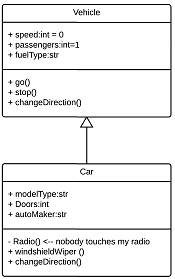
\includegraphics[width=0.25\textwidth]{Bilder/Klassendiagramm/InteraktionVererbung.png}
%\end{wrapfigure}

\begin{minipage}[c]{0.65\textwidth}
	\begin{itemize}
		\item \textbf{Vererbung}: Prozess, bei dem eine Unterklasse die Eigenschaften einer Oberklasse übernimmt, wird auch als Generalisierung bezeichnet. Dargestellt durch eine gerade Verbindungslinie mit geschlossener Pfeilspitze, die auf die Oberklasse zeigt.
	\end{itemize}
\end{minipage}
\hfill
\begin{minipage}[c]{0.25\textwidth}
	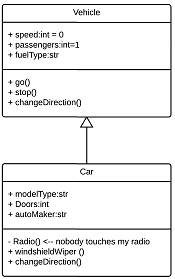
\includegraphics[scale=.7]{Bilder/Klassendiagramm/InteraktionVererbung.png}
\end{minipage}

In diesem Beispiel würde das Objekt \texttt{Car} alle Attribute (\texttt{Geschwindigkeit, Mitfahrerzahl, Treibstoff}) und Methoden (\texttt{Los(), Stop(), Richtungswechsel()}) der Parent-Klasse \texttt{Vehicle} annehmen. Hinzu kämen spezifische Attribute (\texttt{Modelltyp, Türenzahl, Autohersteller}) und Methoden (\texttt{Radio(), \\Scheibenwischer(), Klimaanlage/Heizung()}) der eigenen Klasse. In Klassendiagrammen wird die Vererbung über durchgezogene Linien mit einem geschlossenen, hohlen Pfeil dargestellt.

\begin{itemize}
	\item \textbf{Bidirektionale Assoziation}: die standardmäßige Beziehung zwischen zwei Klassen. Beide Klassen haben Kenntnis von der jeweils anderen und ihrer Beziehung zueinander. Diese Assoziation wird mit einer geraden Linie zwischen zwei Klassen dargestellt.
\end{itemize}

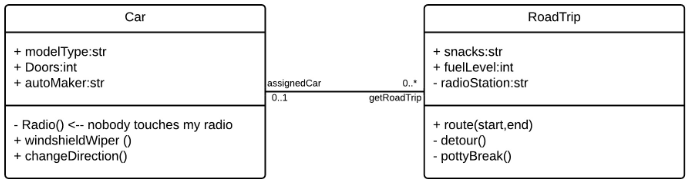
\includegraphics[width=\textwidth]{Bilder/Klassendiagramm/BidirektionaleAssoziation.png}

Im oben genannten Beispiel besteht eine Beziehung zwischen den Klassen \texttt{Car} und \texttt{RoadTrip}. Am Ende der Linie nimmt die Klasse \texttt{Car} die Assoziation \texttt{assignedCar} mit einem Multiplizitätswert von 0..1 an. Wenn die \texttt{RoadTrip}-Instanz existiert, hängt sie also entweder mit einer \texttt{Car}-Instanz oder keiner \texttt{Car}-Instanz zusammen. In diesem Fall wird eine separate \texttt{Wohnwagen}-Klasse mit einem Multiplizitätswert von 0..* benötigt, um zu zeigen, dass eine \texttt{RoadTrip}-Instanz mit mehreren \texttt{Car}-Instanzen zusammenhängen könnte. Da eine \texttt{Car}-Instanz über mehrere Assoziationen von \texttt{getRoadTrip} verfügen könnte (denn ein Auto kann mehrere Strecken zurücklegen), beträgt der Multiplizitätswert 0..*

\subsection{Use-Case-Diagramm (Anwendungsfalldiagramm)}
\label{sec:UseCaseDiagramm}

\subsection{Aktivitätsdiagramm}
\label{sec:Aktivitaetsdiagramm}

\subsection{Sequenzdiagramm}
\label{sec:Sequenzdiagramm}

\subsection{Zustandsdiagramm}
\label{sec:Zustandsdiagramm}